% !TEX program = pdflatex
% Compile with: pdflatex -shell-escape docs/report.tex (for SVG support)
% If you do not have Inkscape, either install it or comment \includesvg and replace with a PNG/PDF.
\providecommand\IfPDFManagementActiveF[1]{#1}

\documentclass[11pt,a4paper]{article}
\usepackage[utf8]{inputenc}
\usepackage[T1]{fontenc}
\usepackage{lmodern}
\usepackage{geometry}
\usepackage{hyperref}
\usepackage{graphicx}
\usepackage{float}
\usepackage{enumitem}
\usepackage{amsmath,amssymb}
\usepackage{caption}
\usepackage{svg} % requires -shell-escape and Inkscape for SVG inclusion

\geometry{margin=1in}
\hypersetup{colorlinks=true,linkcolor=blue,urlcolor=blue,citecolor=blue}

\title{Opis in arhitektura: vizualizacija toka vode (Python in C++)}
\author{Projekt: water\_flow\_visualization}
\date{\today}

\begin{document}
\maketitle

\section*{Povzetek}
Ta dokument opisuje implementacijo vizualizacije toka vode v dveh izvedbah: \texttt{Python} (\texttt{water\_flow\_visualization.py}) in \texttt{C++} (\texttt{water\_flow\_visualization.cpp}). Algoritem temelji na divergencno prostem hitrostnem polju (izpeljanem iz časovno spremenljive tokovne funkcije), polju barvila ("dye"), pol-lagrangevem prenašanju (advekciji) in blagem dušenju, kar daje vodnat, turbulenten videz. Program omogoča živ prikaz (okno) in izvoz animiranega GIF-a.

\section{Pregled algoritma}
\begin{itemize}[noitemsep]
  \item \textbf{Tokovna funkcija} \(\psi(x,y,t)\): kombinacija sinusnih/cosinusnih vzorcev, ki se s časom spreminjajo.
  \item \textbf{Hitrostno polje} \(\vec v = (u,v)\): izračunano kot rotacija tokovne funkcije, \(u = \partial\psi/\partial y,\ v = -\partial\psi/\partial x\), skalirano in rahlo zglajeno (Gauss).
  \item \textbf{Polje barvila} (RGB): inicializirano z modrim odtenkom, šumom in vinjetiranjem za globinski učinek.
  \item \textbf{Advekcija} (pol-lagrangevska): za vsak piksel sledimo poti nazaj po \(\vec v\) in vzorčimo z bilinearno interpolacijo.
  \item \textbf{Dušenje in barvno ravnotežje}: mešanica trenutnega barvila z osnovnim (0.5\%).
  \item \textbf{Izhod}: posodabljanje okna (neobvezno) in sestavljanje GIF-a s podano hitrostjo sličic (FPS).
\end{itemize}

\begin{figure}[H]
  \centering
  % Avoid LaTeX overlay from Inkscape (underscores in labels can break compilation)
  % \includesvg[inkscapelatex=false,width=0.95\linewidth]{flowchart}
  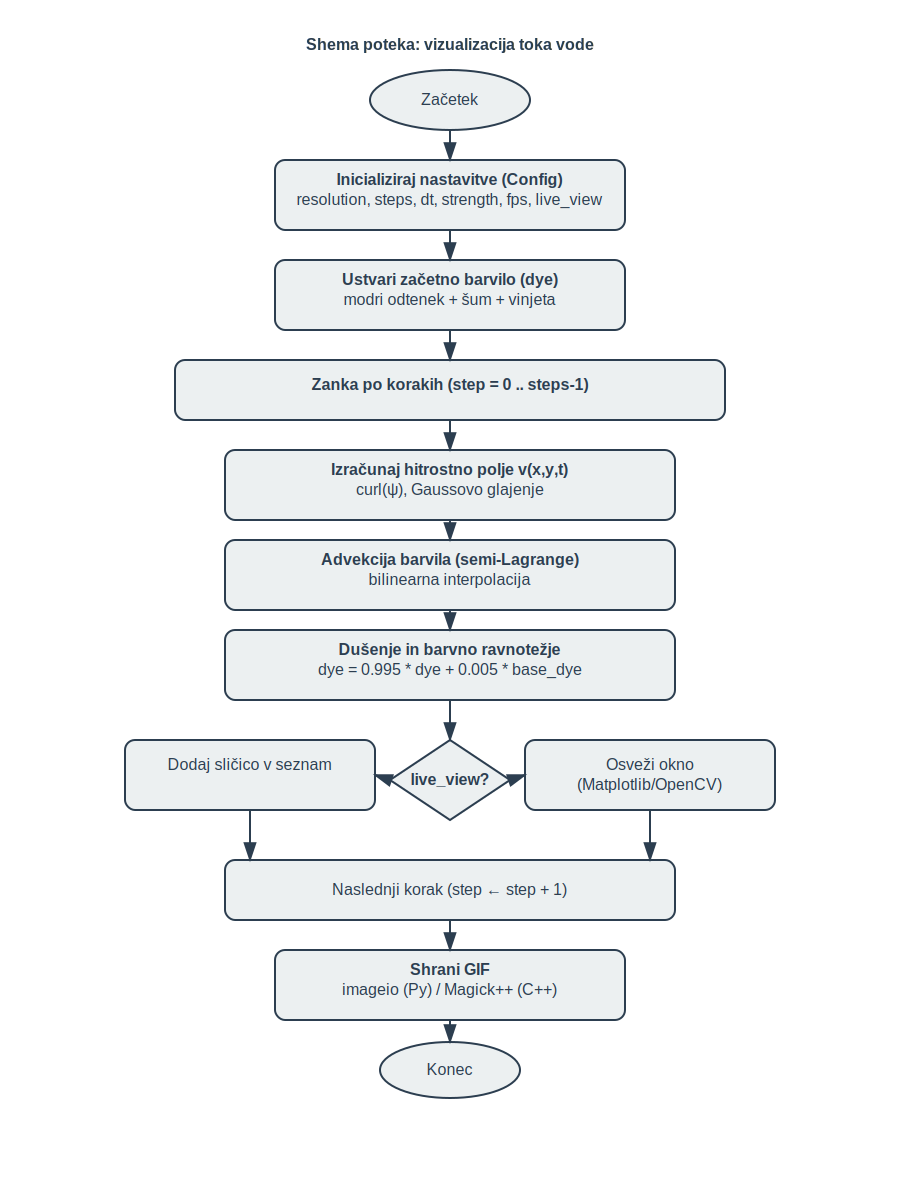
\includegraphics[width=0.95\linewidth]{flowchart.png}
  \caption{Shema poteka algoritma (flowchart).}
\end{figure}

\section{Python: \texttt{water\_flow\_visualization.py}}
\subsection*{Ključne komponente}
\begin{itemize}[noitemsep]
  \item \textbf{\texttt{SimulationConfig}}: nastavitve (\texttt{resolution, steps, dt, strength, fps, live\_view, gif\_name, output\_dir}).
  \item \textbf{Tokovna funkcija in hitrostno polje}: \texttt{stream\_function}, \texttt{velocity\_field}, \texttt{gaussian\_blur}.
  \item \textbf{Vzorčenje in advekcija}: \texttt{bilinear\_sample}, \texttt{advect}.
  \item \textbf{Inicializacija barvila}: \texttt{create\_initial\_dye} (modri toni + Gaussov šum + vinjeta).
  \item \textbf{Zanka simulacije}: izračun \(\vec v\), advekcija, dušenje, osvežitev okna (če je omogočeno), zbiranje sličic.
  \item \textbf{Izvoz}: \texttt{imageio.mimsave} za GIF; \texttt{matplotlib} za živ prikaz.
\end{itemize}

\subsection*{Zagon}
\begin{verbatim}
python water_flow_visualization.py --fps=90 --strength=1.2 --no-live-view
\end{verbatim}
Podprti so tudi preprosti preglasi nastavitev v obliki \texttt{--key=value}.

\section{C++: \texttt{water\_flow\_visualization.cpp}}
\subsection*{Ključne komponente}
\begin{itemize}[noitemsep]
  \item \textbf{\texttt{Config}}: enake nastavitve kot v Pythonu.
  \item \textbf{Tok in hitrost}: \texttt{streamFunction}, \texttt{buildVelocityField}, \texttt{gaussianBlur} (ločljivi 1D filtri).
  \item \textbf{Advekcija}: \texttt{advect} z bilinearno interpolacijo.
  \item \textbf{Inicializacija}: \texttt{createInitialDye} (modra baza + šum + vinjeta).
  \item \textbf{Živ prikaz (neobvezno)}: OpenCV okno (če je \texttt{USE\_OPENCV}); posodobitev vsako sličico.
  \item \textbf{GIF izvoz}: prek Magick++ (ImageMagick) se sličice zapišejo v animacijo z želenim FPS.
\end{itemize}

\subsection*{Gradnja (CMake)}
\begin{verbatim}
cmake -S . -B build -DWATER_FLOW_USE_OPENCV=ON \
  -DOpenCV_DIR="C:\\Libraries\\opencv-4.10.0\\Build" \
  -DImageMagick_INCLUDE_DIRS="C:\\Program Files\\ImageMagick-7.1.2-Q16-HDRI\\include" \
  -DImageMagick_LIBRARIES="C:\\Program Files\\ImageMagick-7.1.2-Q16-HDRI\\lib\\CORE_RL_Magick++_.lib; \\
    C:\\Program Files\\ImageMagick-7.1.2-Q16-HDRI\\lib\\CORE_RL_MagickCore_.lib; \\
    C:\\Program Files\\ImageMagick-7.1.2-Q16-HDRI\\lib\\CORE_RL_MagickWand_.lib"
cmake --build build --config Release
\end{verbatim}
Zagon: \texttt{build\\Release\\water\_flow\_cpp.exe --fps=90} (dodajte \texttt{--no-live-view} za "headless").

\section{Parametri in priporočila}
\begin{itemize}[noitemsep]
  \item \textbf{\texttt{resolution}}: velikost slike (privzeto 512). Višje vrednosti so počasnejše.
  \item \textbf{\texttt{steps}}: število sličic (trajanje GIF-a).
  \item \textbf{\texttt{dt}}: korak časa za advekcijo (stabilnost/ostrost vzorca).
  \item \textbf{\texttt{strength}}: skala hitrosti; višje pomeni izrazitejši vrtinci.
  \item \textbf{\texttt{fps}}: hitrost GIF-a in predogleda.
  \item \textbf{\texttt{live\_view}}: omogoči/izključi okno za predogled (OpenCV/Python Matplotlib).
\end{itemize}

\section{Razlike med izvedbama}
\begin{itemize}[noitemsep]
  \item \textbf{Odvisnosti}: Python uporablja \texttt{numpy/matplotlib/imageio}, C++ pa \texttt{Magick++} in po želji \texttt{OpenCV}.
  \item \textbf{Hitrost}: C++ je običajno hitrejši; Python je preprostejši za prilagoditve.
  \item \textbf{Vizualno}: algoritmi so usklajeni; zaradi numeričnih razlik so možne manjše razlike v teksturah.
\end{itemize}

\section{Izhod kot PDF}
Za vključitev SVG uporabite \texttt{-shell-escape} in nameščen Inkscape:
\begin{verbatim}
pdflatex -shell-escape docs/report.tex
\end{verbatim}
Če SVG pretvorba ni na voljo, zamenjajte \verb|\includesvg{flowchart}| z \verb|\includegraphics| na PNG/PDF različico diagrame (ali uporabite TikZ).

\end{document}
